\documentclass[final,hyperref={pdfpagelabels=false}]{beamer}
\newcommand{\citet}[1]{\citeA{#1}}
\newcommand{\citep}[1]{\cite{#1}}


\mode<presentation>
  {
  \usetheme{pennstate}
  %\usetheme{Dreuw}
  }
  \usepackage{times}
  \usepackage{amsmath,amsthm, amssymb, latexsym, apacite}
  \boldmath
  \usepackage[english]{babel}
  \usepackage[latin1]{inputenc}
  \usepackage[orientation=portrait,size=custom,width=60.96,height=91.44]{beamerposter}

  %%%%%%%%%%%%%%%%%%%%%%%%%%%%%%%%%%%%%%%%%%%%%%%%%%%%%%%%%%%%%%%%%%%%%%%%%%%%%%%%%5
  \graphicspath{{figures/}}
  \title[Symmetry Perception]{Human Perception of 2D Symmetry}
  \author[Cole \& Reitter \& Liu]{Jeremy Cole, David Reitter, and Yanxi Liu}
  \institute[Penn State]{The Pennsylvania State University}
  \date{2016}



  %%%%%%%%%%%%%%%%%%%%%%%%%%%%%%%%%%%%%%%%%%%%%%%%%%%%%%%%%%%%%%%%%%%%%%%%%%%%%%%%%5
  \begin{document}
  \begin{frame}{} 
    \vfill
    %\begin{block}{\LARGE Abstract}
    %  \begin{abstract}
This paper investigates human ability to innately perceive multiple different features of symmetry. While most work has focused on simple bilateral reflection symmetry, these experiments make a case that humans can perceive much more than that. By using a set of images that each conform to one of the seventeen wallpaper groups, we investigate which wallpapers groups are easiest and most difficult to tell apart. This allows us to provide evidence that rotation and reflection are not sufficient in explaining perception of symmetry, challenging some prevailing notions.

\textbf{Keywords:} 
visual perception; symmetry
\end{abstract}
    %\end{block}    
	\begin{columns}[t]
	\begin{column}{.12\linewidth}
	    	    		\begin{block}{Reflection}
	    	    		 \section{Background}
\begin{figure}
\centering
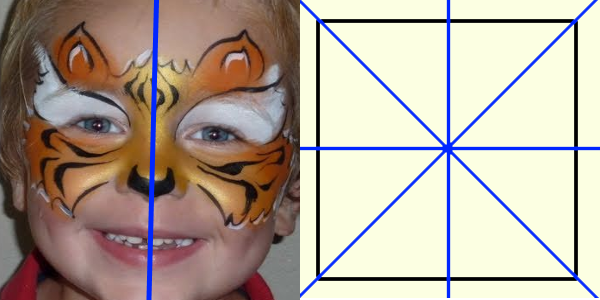
\includegraphics[height=0.05\textheight, width=0.9\columnwidth]{reflection}
\caption{Characterized by the number and placement of its axes}
\label{ref}
\end{figure}
	    	    		\end{block}
	    	    		\vfill
	    	    		\begin{block}{Rotation}
	    	    		\begin{figure}
\centering
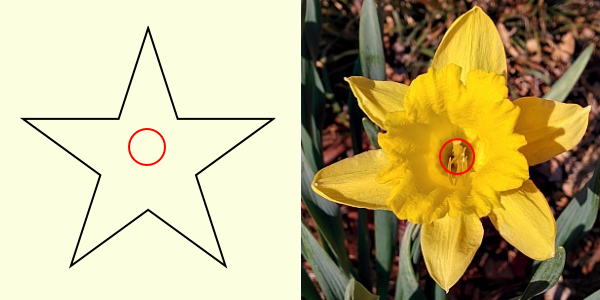
\includegraphics[width=0.9\columnwidth]{rotation}
\caption{Characterized by the number of rotation angles}
\label{rot}
\end{figure}
	    	    		\end{block}
	    	    	\end{column}
	    	    	\begin{column}{.12\linewidth}
	    	    		\begin{block}{Glide Refl}
	    	    			\begin{figure}
\centering
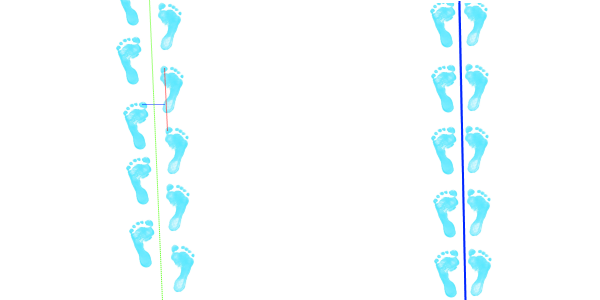
\includegraphics[width=0.9\columnwidth]{glide}
\caption{Characterized by the number and location of the axes}
\label{glide}
\end{figure}				 
	    		  		\end{block}
	    		  			\vfill
	    	    		\begin{block}{Translation}
	    	    	    		\begin{figure}
\centering
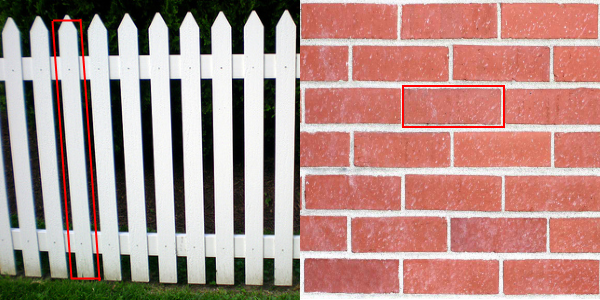
\includegraphics[height=0.05\textheight, width=0.9\columnwidth]{translation}
\caption{Characterized by the repeating shape}
\label{trans}
\end{figure}  
	    	    	    \end{block}
	    	    	    	\end{column}
		\begin{column}{0.24\linewidth}
			\begin{block}{Symmetry}
    		\section{Introduction}
Symmetry has oft been studied as a feature of visual perception and attention (see \citet{review} for a review). However,  the cognitive science community has focused primarily on bilateral reflection symmetry. The question is: why? This study 
% 
{\it seeks to examine why researchers have largely ignored other types of symmetry and }{\bf your paper doesn't actually answer this somewhat irrelevant question.}
will demonstrate that a broader conceptualization of symmetry is useful to studies of human perception and attention.

Symmetry refers to a transformation of an object or image that leaves it with the exact same appearance. There are four primitive types of symmetry: rotation, reflection, glide reflection, and translation. The vernacular term symmetry generally refers to reflection, with the majority of studies focused on bilateral reflection, where the axis is in the center of the object or image.

This paper will focus on \textit{wallpapers}: a type of infinitely repeating symmetric image that is characterized by a specific set of symmetries. First, we will provide the reader with the necessary background to understand this conceptualization, then we will review past work on symmetry, and then we will present a set of findings that show humans are quite adept at detecting other types of symmetry besides bilateral reflection.




    		\end{block}
    	\end{column}
    	    	\begin{column}{.24\linewidth}
    	   			 \begin{block}{Wallpaper Groups}
\begin{figure}[!ht]
\centering
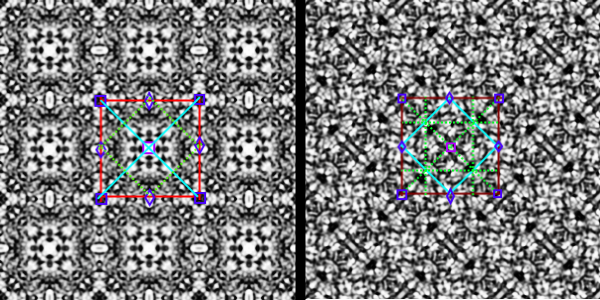
\includegraphics[height=0.074\textheight, width=0.9\columnwidth]{ann_images}
\caption{Different Groups: On the left is P4M, on the right is P4G.}
\label{P4GvP4M}
\end{figure}

\begin{figure}[!ht]
\centering
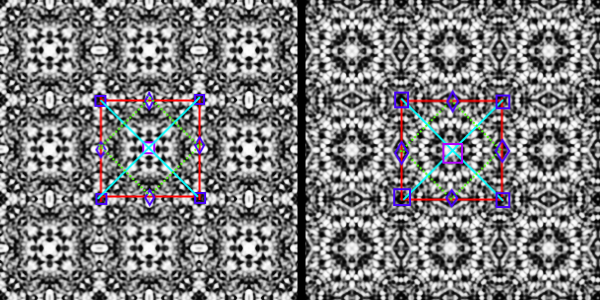
\includegraphics[height=0.074\textheight, width=0.9\columnwidth]{ann_images_same}
\caption{Same Groups: Both P4M.}
\label{P4MvP4M}
\end{figure}
\end{block}  
    	    	\end{column}
    	  \begin{column}{0.24\linewidth}
    	  	\begin{block}{Wallpapers}
    	  		We use \emph{wallpapers} to create images that use combinations of these symmetry types. Wallpapers are two-dimensional images made from an infinitely repeating symmetric \textit{tile}. These tiles are characterized by a specific set of symmetries. There are exactly seventeen wallpaper groups, as has been well-known for over a hundred years \citep{wallpaper-proof}. In other words, every two-dimensional repeating image has one of seventeen sets of symmetries. These wallpapers can be arranged in a hierarchy, which we argue relates to how they are perceived.
    	  	\end{block}
    	  \end{column}
    \end{columns}
    \vfill
    
    \begin{columns}[t]
    \begin{column}{.32\linewidth}
        	       		\begin{block}{Wallpaper Group Features}
        	       		 	\begin{table}[!ht]
    \centering
    \resizebox{\columnwidth}{!}{%
    \begin{tabular}{|l|c|c|c|c|c|c|c|c|c|}
    \hline
    Group & 2-fold & 3-fold & 4-fold & 6-fold & $T_1$ & $T_2$ & $D_1$ & $D_2$ &  tile \\ \hline
    P1 & F & F & F & F & None & None & None & None & O \\ \hline
    P2 & T & F & F & F & None & None & None & None & O \\ \hline
    PM & F & F & F & F & Refl & None & None & None & Re \\ \hline
    PG & F & F & F & F & Glide & None & None & None & Re \\ \hline
    CM & F & F & F & F & None & None & Refl & None & Rh \\ \hline
    PMM & T & F & F & F & Glide & Refl & None & None & Re \\ \hline
    PMG & T & F & F & F & Glide & Refl & None & None & Re \\ \hline
    PGG & T & F & F & F & Glide & Glide & None & None & Re \\ \hline
    CMM & T & F & F & F & None & None & Refl & Refl & Rh \\ \hline
    P4 & T & F & T & F & None & None& None & None & S \\ \hline
    P4M & T & F & T & F & Refl & Refl & Refl & Refl & S \\ \hline
    P4G & T & F & T & F & Glide & Glide & Refl & Refl & S \\ \hline
    P3 & F & T & F & F & None & None & None & None & H \\ \hline
    P3M1 & F & T & F & F & None & None & Refl& None & H \\ \hline
    P31M & F & T & F & F & Refl & Refl & Refl & None & H \\ \hline
    P6 & T & T & F & T & Refl & None & None & None & H \\ \hline
    P6M & T & T & F & T & Refl & Refl & Refl & Refl & H \\ \hline
    \end{tabular}%
    }
    \caption{Wallpaper groups represented as their symmetries. The first four columns are whether the group has that type of rotation symmetry. The second four columns refer to the four main axes on the tile. (Refl=Reflection, Glide=Glide Reflection, Re=Rectangular, Rh=Rhombic, O=Oblique, S=Square, H=Hexagonal)}
    \label{sym-tab}
\end{table}
        	       		 \end{block}
        	       		 
        	       	\end{column}
    	\begin{column}{.24\linewidth}
    	\begin{block}{Methods}
    	    	We recruited 106 subjects from the Amazon Mechanical Turk platform to compare among the wallpaper groups. Their basic task was to match two wallpapers from the same group. The third image could be from any of the other sixteen groups. In this way, we could distinguish how difficult it is for humans to tell the groups apart. Further, we only allowed each participant five seconds, in order to force them to rely on perceptual, rather than analytical, processes. All subjects were compensated for their time, though 12 were excluded for behavior consistent with not taking the task seriously. 
    	    \end{block}
    	\end{column}
    	\begin{column}{.40\linewidth}
    	\begin{block}{Task Screenshot}
    		\section{Figures}

All artwork must be very dark for purposes of reproduction and should
not be hand drawn. Number figures sequentially, placing the figure
number and caption, in 10~point, after the figure with one line space
above the caption and one line space below it, as in
Figure~\ref{sample-figure}. If necessary, leave extra white space at
the bottom of the page to avoid splitting the figure and figure
caption. You may float figures to the top or bottom of a column, or
set wide figures across both columns.

\begin{figure}[ht]
\begin{center}
\fbox{CoGNiTiVe ScIeNcE}
\end{center}
\caption{This is a figure.} 
\label{sample-figure}
\end{figure}
    	\end{block}
    	\end{column}
    		
    \end{columns}
    \begin{columns}[t]
       \begin{column}{.31\linewidth}
       \begin{block}{Wallpaper Hierarchy}
               	      		 	\begin{figure}[!ht]
\centering
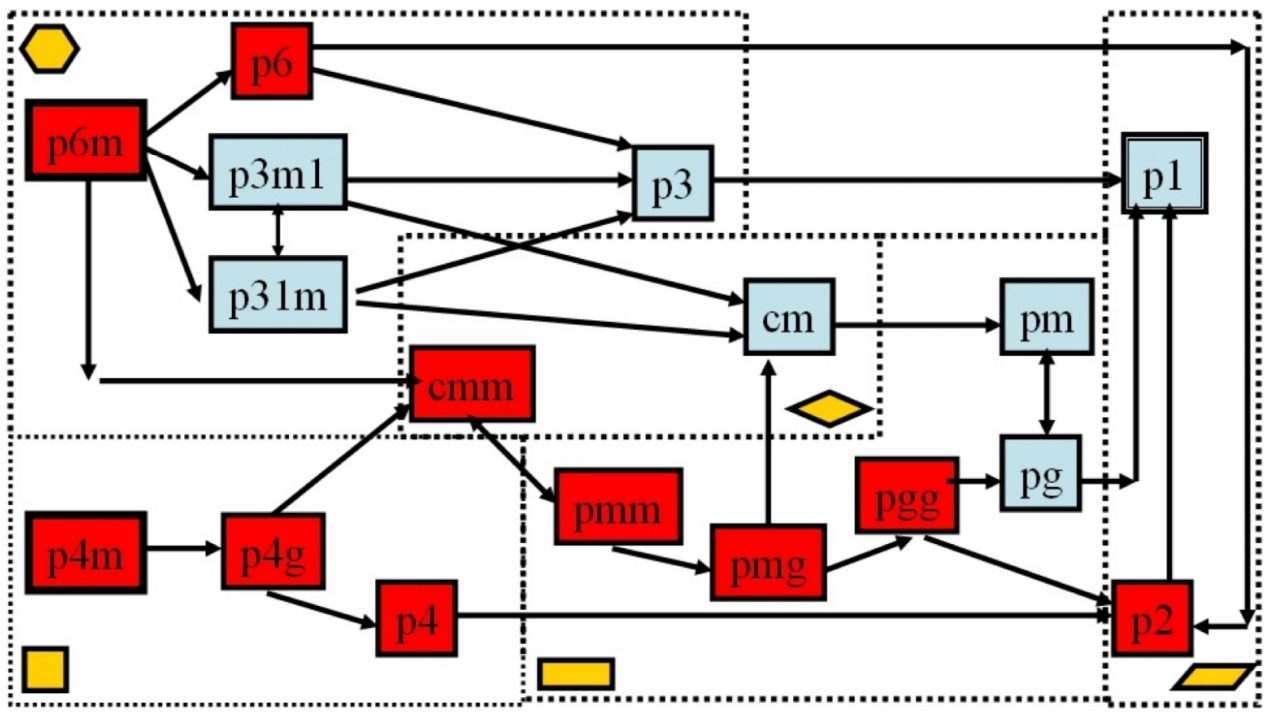
\includegraphics[width=0.9\columnwidth]{Yanxi_Graph}
\caption{If an arrow points from any given box, $A$, toward any given box $B$, that means that $B$'s symmetries are subset of $A$'s symmetries.}
\label{graph}
\end{figure}
               	      		 	%\begin{block}{Statistics}
               	    			%We used simple binomial t-tests to determine how accurate humans were at distinguishing among every wallpaper group. We also used a Linear Mixed Effects Model to determine what drives the variance in distinguishing between two pairs of wallpapers. Our features in the model consisted of the symmetries as defined by the group-theoretic analysis of the wallpaper groups. We additionally considered \textit{subgroup distance}, an aggregate measure referring to the shortest path in the subgroup graph, and \textit{tile shape}, the piece of the image that is infinitely translated.
               	    			%\end{block}
               	       		\end{block}
               	       		\begin{block}{Most Difficult Comparison}
               	       		      			\begin{figure}[!ht]
\centering
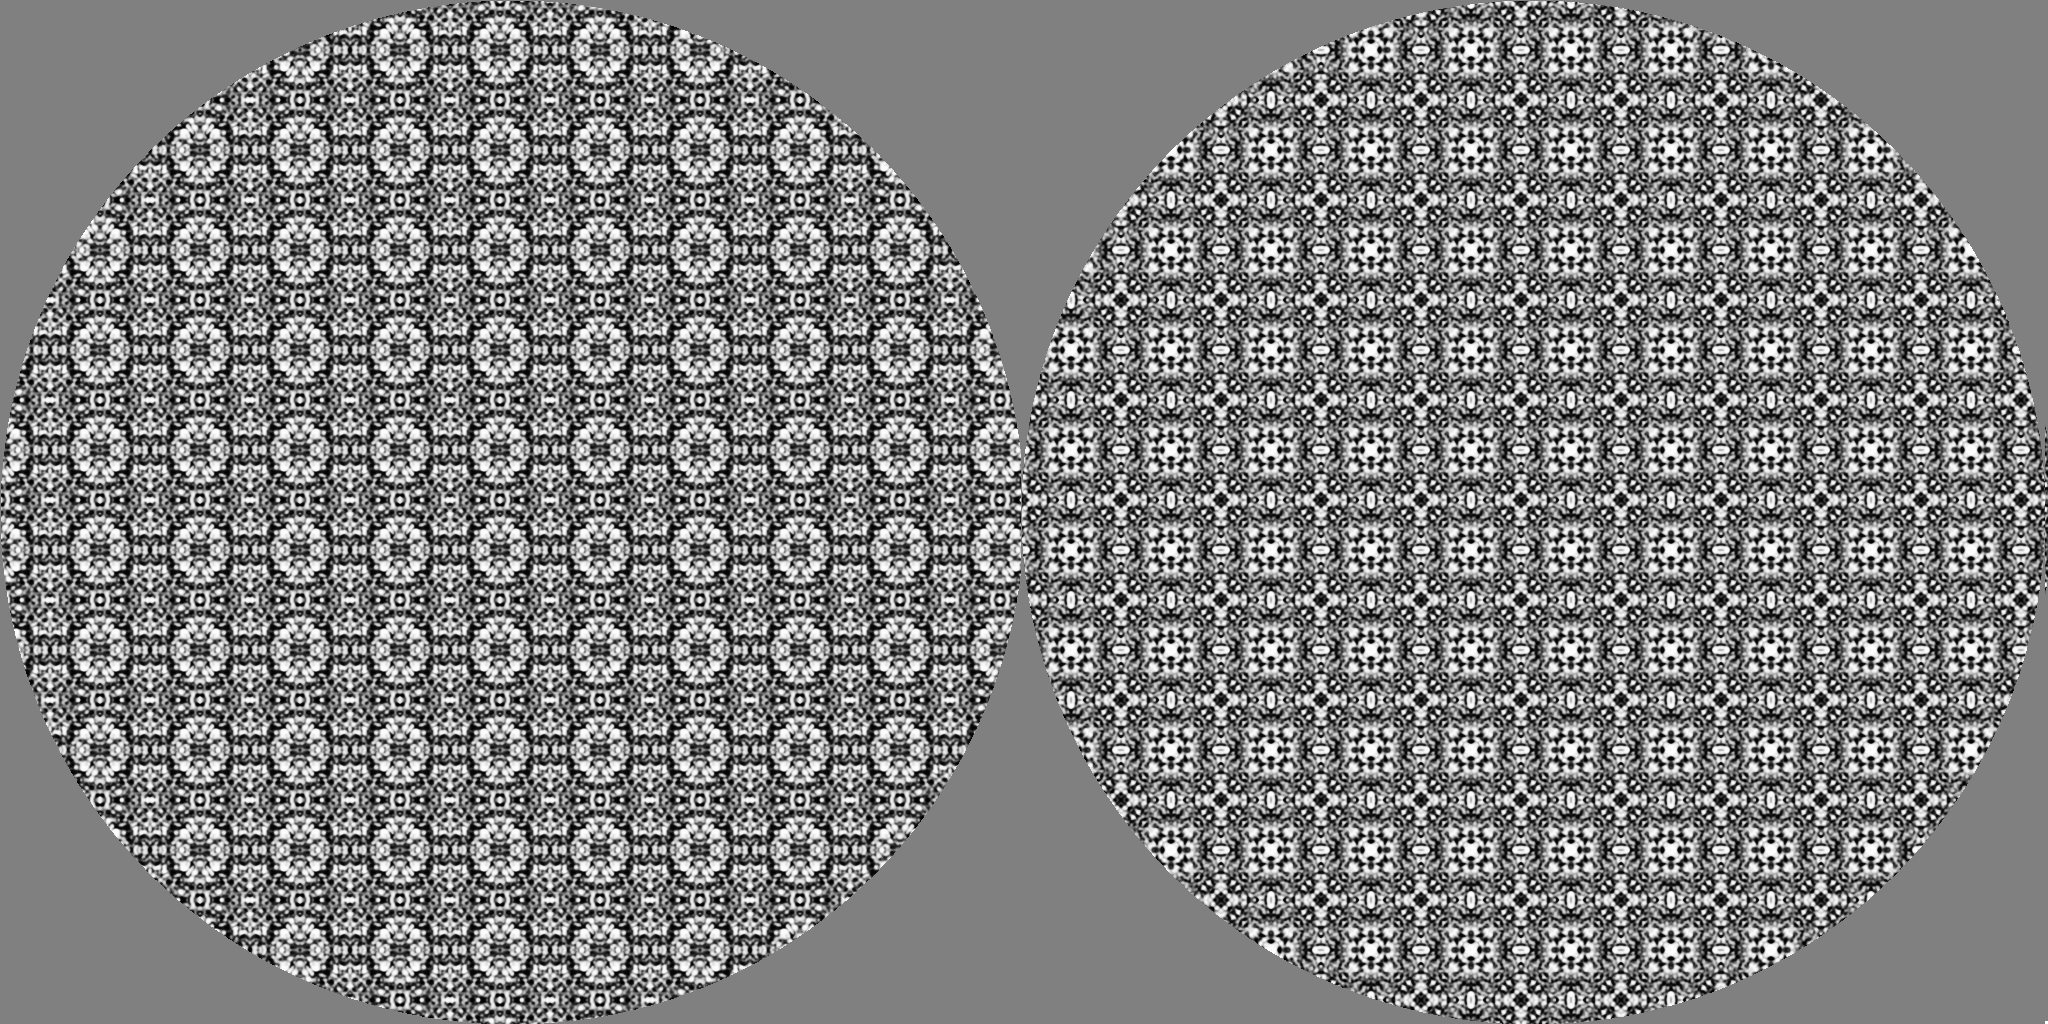
\includegraphics[width=0.9\columnwidth]{pmmp4m}
\caption{PMM on the left, P4M on the right (look at positive diagonal).}
\label{pmmp4m}
\end{figure}
               	       		      		\end{block}
       \end{column}
       	\begin{column}{.35\linewidth}
       		\begin{block}{Accuracy Chart}
      			\section{Analysis}
Our two basic research questions were addressed individually.

\subsection{Question 1}
To answer the first research question, we can rely on subjects' accuracy in distinguishing the two groups. We calculated this by combining the results for each as the distracter and the target. Then, we aggregated all the subjects and took the percentage that was correct. Our hypothesis was that participants can tell apart every group from every single group. To test this, we simply looked at the lowest percentage. We modeled the data as a binomial distribution with $\pi=0.5$, assuming the subjects were required to guess. Importantly, as there were $136$ tests of significance that took place, the chance of each one being significant at the $0.05$ level if they were on the edge of significance is $0.09\%$. 

In our study, the most difficult for participants was the distinction between “p4mm” and “pmm”. Across the 96 participants, only 56.8\% of trials were successful. On a single-tailed binomial distribution, there is a p-value of $0.06$ on that number of trials. While this misses the classical $0.05$ marker for significance, every single other group by group comparison meets it. Therefore, we find it likely that with more subjects, every group would have shown itself to be statistically distinguishable. The average accuracy fell right around 76.8\%, which is clearly far better than people would perform if they were at all guessing. Further, due to the number of significance tests, there would be some natural variation in any specific test.

\subsection{Question 2}
\textbf{This part I still need to do based on model comparison}
To answer our second question, we used a Linear Mixed Effects Regression model. Since we wanted to predict what caused the subjects to choose correctly, we used accuracy as the response variable. Thus, the first step was to change each task to its own record. Then, each feature we considered could have a positive of negative impact on the accuracy, represented as a slope.

Each task was boiled down to a comparison of the two symmetry group’s features. These features were whether or not the groups of the target and distracter images had the same tile shape, whether they both have reflection, whether they both have glide reflection, and whether they have the same rotation order. Lastly, we also included the value for the shortest path on the subgroup relation graph; for instance, the distance from “p6m” to “p6” is 1. While each of the first four refer to some basic feature of symmetry, the graph distance is included as somewhat of an alternative theory. In short, it would posit that humans perceive symmetry very closely to its mathematical analysis, instead of as a collection of individual symmetries.

We used two random effect variables, which represent uncontrolled aspects of the model. The first is the actual participant who performed the task, which obviously has some effect on the accuracy. The second is the actual images they looked at: each participant was presented a different combination of the 85 total images we used. Thus, the combination they looked at could also play a role, even if each image was from the same group.

\begin{figure}[!ht]
\centering
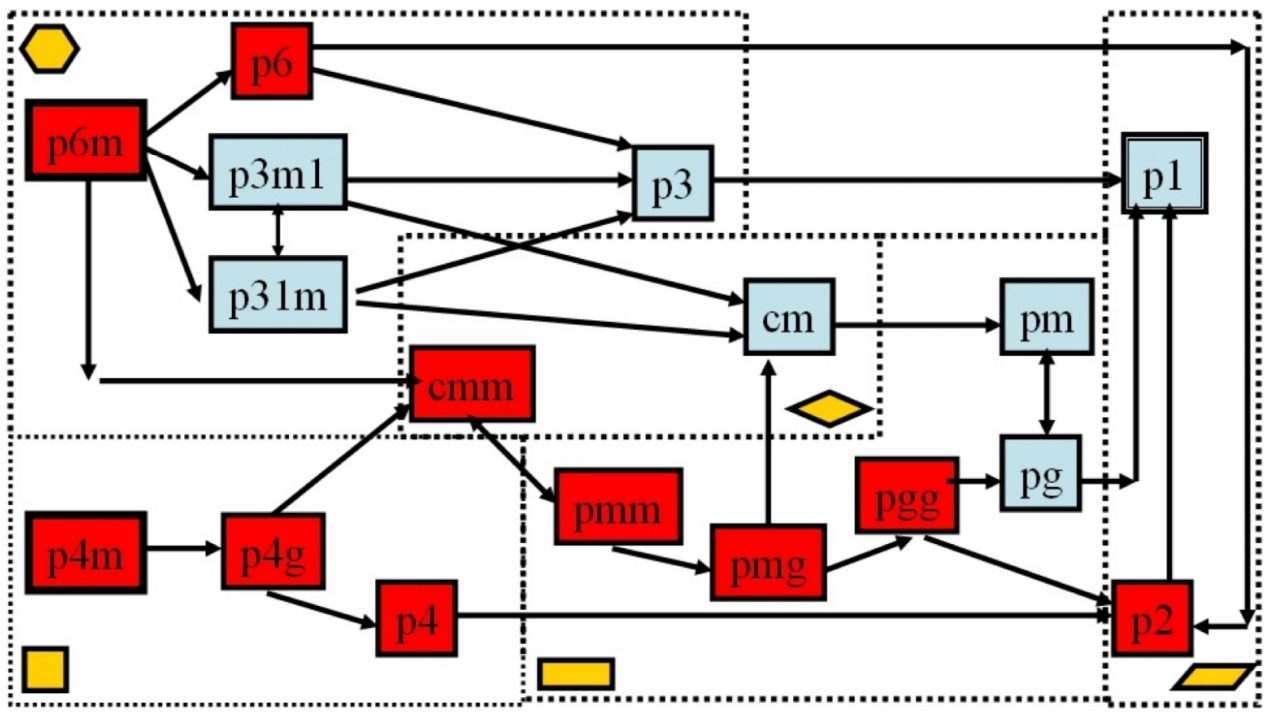
\includegraphics[width=0.9\columnwidth]{Yanxi_Graph}
\label{graph}
\caption{The subgroup relation graph}
\end{figure}

No interaction terms were considered, so the equation was simply: 

\[\mathrm{acc} \sim \mathrm{rot}+\mathrm{ref}+\mathrm{gref}+\mathrm{tile}+\mathrm{distance}+(1\mid \mathrm{subject})+(1 \mid \mathrm{task})\]

To be clear, accuracy (acc) in each record was 1 or 0. Rotation (rot), reflection (ref), glide reflection (gref), and tile shape (tile) were all either true or false based on whether the target image had the same value as the distracter image. The subject and the task were numeric based on their ID in the database. Please see Table~\ref{results} for a break-down of the results.

This shows that tile shape, glide reflection, and distance were all significant in determining accuracy. However, neither reflection or rotation are.

\begin{table}
\centering
\begin{tabular}{|l|ccc|}
\hline
& Estimate & Std. Error & t value \\ \hline
Rotation& 0.005650& 0.007742& 0.73 \\ \hline
Reflection& -0.004545& 0.005768& -0.79 \\ \hline
Glide Reflection& 0.06854& 0.005382& 3.13* \\ \hline
Tile& -0.030277& 0.006732& -3.87* \\ \hline 
Distance& 0.028984& 0.002781& 10.42* \\ \hline
\end{tabular}
\label{results}
\caption{Fixed Effects}
\end{table}      			
      		\end{block}
      		
      			\begin{block}{Conclusions}
      		     			The best model (by AIC ) included subgroup distance, the $T_1$ axis (lateral reflection symmetry), the $D_1$ axis (the positive diagonal), 4-fold and 3-fold rotation. Our participants were quite good at distinguishing among the groups, though accuracy varied. \textit{Subgroup distance} was a significant and improved the AIC of every model. This could mean that human pattern analysis at the rapid heuristic level is similar to the mathematical level. 
      		     		\end{block}
      		     	
       	\end{column}
       	\begin{column}{.30\linewidth}
      		\begin{block}{Fixed Effects}
   				\begin{table}
\centering
\begin{tabular}{|l|rrrl|}
\hline
& Estimate & Std. Error & z value & Pr$(<|z|)$  \\ \hline
(Intercept) & 0.95971 &  0.09950 & 9.645 & $<0.00001$* \\ \hline
T1 & -0.24795 &  0.04150 & -5.975 &  $<0.00001$* \\ \hline
T2 & -0.07746 & 0.04026 & -1.924 & 0.0544 \\ \hline
D1 & -0.31416 & 0.04063 & -7.732 &  $<0.00001$* \\ \hline
D2 & 0.10197 & 0.04431 & 2.301 & 0.0214* \\ \hline
2fold & 0.01214 & 0.03540 & 0.343 & 0.7316 \\ \hline
3fold & -0.18056 & 0.04197 & -4.302 & $0.00017$* \\ \hline
4fold & 0.32353 & 0.04282 & 7.555 & $<0.00001$* \\ \hline
6fold & -0.07538 & 0.04484 & -1.711 & 0.0870 \\ \hline
tile & -0.07891 & 0.05556 & -1.420 & 0.1555 \\ \hline
distance & 0.22420 & 0.01872 & 11.978 & $<0.00001$*\\ \hline
\end{tabular}
\caption{Logistic Linear Mixed-Effects model predicting accuracy with by-item and by-subject random intercepts. }
\label{fixeff}
\end{table}		
     		\end{block}
     			\begin{block}{Bibliography}
     		      		     			\bibliographystyle{apacite}
     		      		     			\renewcommand*{\bibliographytypesize}{\small}
     		      		     			%\fontsize{42pt}{10pt}
     		      		     			\bibliography{symmetry2,symmetry3,symmetry,perception,reflection,yanxibook}
     		      		     		\end{block}
     	
     	\end{column}
    \end{columns}
  \end{frame}

\end{document}


%%%%%%%%%%%%%%%%%%%%%%%%%%%%%%%%%%%%%%%%%%%%%%%%%%%%%%%%%%%%%%%%%%%%%%%%%%%%%%%%%%%%%%%%%%%%%%%%%%%%
%%% Local Variables: 
%%% mode: latex
%%% TeX-PDF-mode: t
%%% End:
